\documentclass[a4paper, 11pt]{article}
\usepackage{amsgen,amsmath,amstext,amsbsy,amsopn,amssymb,amscd,amsthm}
\usepackage{listings}
\usepackage{setspace}
\usepackage{graphicx}
\usepackage{epstopdf}
\usepackage{hyperref}
\usepackage{dcolumn}% Align table columns on decimal point
\usepackage{bm}% bold math
\usepackage{booktabs}
\usepackage[OT1]{fontenc}
\usepackage[]{natbib}
\usepackage{pdfsync}
\usepackage{color}
\usepackage{parskip}
\usepackage{multirow}
\usepackage{natbib}
\usepackage[utf8]{inputenc}
\usepackage{hyperref}
\hypersetup{
  colorlinks   = true, %Colours links instead of ugly boxes
  urlcolor     = blue, %Colour for external hyperlinks
  linkcolor    = blue, %Colour of internal links
  citecolor   = red %Colour of citations
}

% Default fixed font does not support bold face
\DeclareFixedFont{\ttb}{T1}{txtt}{bx}{n}{12} % for bold
\DeclareFixedFont{\ttm}{T1}{txtt}{m}{n}{12}  % for normal

% Custom colors
\usepackage{color}
\definecolor{deepblue}{rgb}{0,0,0.5}
\definecolor{deepred}{rgb}{0.6,0,0}
\definecolor{deepgreen}{rgb}{0,0.5,0}

\usepackage{listings}

% Python style for highlighting
\newcommand\pythonstyle{\lstset{
language=Python,
basicstyle=\ttm,
otherkeywords={self},             % Add keywords here
keywordstyle=\ttb\color{deepblue},
emph={MyClass,__init__},          % Custom highlighting
emphstyle=\ttb\color{deepred},    % Custom highlighting style
stringstyle=\color{deepgreen},
frame=tb,                         % Any extra options here
showstringspaces=false            % 
}}


% Python environment
\lstnewenvironment{python}[1][]
{
\pythonstyle
\lstset{#1}
}
{}

% Python for external files
\newcommand\pythonexternal[2][]{{
\pythonstyle
\lstinputlisting[#1]{#2}}}

% Python for inline
\newcommand\pythoninline[1]{{\pythonstyle\lstinline!#1!}}


\setlength{\topmargin}{-0.5in}
\setlength{\oddsidemargin}{0in}
\setlength{\evensidemargin}{0in}
\setlength{\textheight}{9in}
\setlength{\textwidth}{6.5in}
\setlength{\footskip}{0.2in}


\newtheorem{theorem}{Theorem}[section]
\newtheorem{corollary}{Corollary}[section]
\newtheorem{proposition}{Proposition}[section]
\newtheorem{lemma}{Lemma}[section]
\newtheorem{example}{Example}[section]
\newtheorem{definition}{Definition}[section]

\newcommand{\thmref}[1]{Theorem~\ref{#1}}
\newcommand{\propref}[1]{Proposition~\ref{#1}}
\newcommand{\corref}[1]{Corollary~\ref{#1}}
\newcommand{\lemref}[1]{Lemma~\ref{#1}}
\newcommand{\secref}[1]{\S\ref{#1}}
\newcommand{\figref}[1]{Figure~\ref{#1}}


\newcommand{\wt}{\widetilde}

\newcommand{\fdp}{\textsc{fdp}}
\newcommand{\fdr}{\textsc{fdr}}
\newcommand{\fnr}{\textsc{fnr}}
\newcommand{\fnp}{\textsc{fnp}}
\newcommand{\mfdr}{m\textsc{fdr}}
\newcommand{\mfnr}{m\textsc{fnr}}

\newcommand{\sor}{\textsc{or}}

\newcommand{\Cov}{\mathrm{Cov}}
\newcommand{\Cor}{\mathrm{Cor}}
\newcommand{\diag}{\mathrm{diag}}
\newcommand{\Var}{\mathrm{Var}}
\newcommand{\sgn}{\mathrm{sgn}}

\newcommand{\normal}{\mathrm{N}}

\newcommand{\etc}{\textit{etc}.}
%\newcommand{\etal}{\textit{et al}}
\newcommand{\ie}{\textit{i.e.}}
\newcommand{\eg}{\textit{e.g.}}
\newcommand{\iid}{\textit{i.i.d}}
\newcommand{\vs}{\textit{vs.}}

\newcommand{\trans}{\mathrm{T}}
\newcommand{\ud}{\,\mathrm{d}}
\newcommand{\uH}{\,\mathrm{H}}
\newcommand{\EE}{\mathbb{E}}
\newcommand{\PP}{\mathbb{P}}
\newcommand{\RR}{\mathbb{R}}
\newcommand{\NN}{\mathbb{N}}
\newcommand{\Or}{\mathcal{O}}
\newcommand{\Ir}{\mathcal{I}}
\newcommand{\Ar}{\mathcal{A}}
\newcommand{\Br}{\mathcal{B}}
\newcommand{\Cr}{\mathcal{C}}
\newcommand{\Dr}{\mathcal{D}}
\newcommand{\Er}{\mathcal{E}}
\newcommand{\Mr}{\mathcal{M}}
\renewcommand{\Or}{\mathcal{O}}
\renewcommand{\Pr}{\mathcal{P}}
\newcommand{\Rr}{\mathcal{R}}
\newcommand{\Ur}{\mathcal{U}}
\newcommand{\Vr}{\mathcal{V}}
\newcommand{\Sr}{\mathcal{S}}
\newcommand{\Cf}{\mathfrak{C}}
\newcommand{\Sf}{\mathfrak{S}}

\newcommand{\va}{\boldsymbol{a}}
\newcommand{\vA}{\boldsymbol{A}}
\newcommand{\vb}{\boldsymbol{b}}
\newcommand{\vc}{\boldsymbol{c}}
\newcommand{\vD}{\boldsymbol{D}}
\newcommand{\ve}{\boldsymbol{e}}
\newcommand{\vh}{\boldsymbol{h}}
\newcommand{\vi}{\boldsymbol{i}}
\newcommand{\vk}{\boldsymbol{k}}
\newcommand{\vK}{\boldsymbol{K}}
\newcommand{\vI}{\mathbf{I}}
\newcommand{\vL}{\boldsymbol{L}}
\newcommand{\vP}{\boldsymbol{P}}
\newcommand{\vp}{\boldsymbol{p}}
\newcommand{\vr}{\boldsymbol{r}}
\newcommand{\vu}{\boldsymbol{u}}
\newcommand{\vV}{\boldsymbol{V}}
\newcommand{\vx}{\boldsymbol{x}}
\newcommand{\vX}{\boldsymbol{X}}
\newcommand{\vy}{\boldsymbol{y}}
\newcommand{\vY}{\boldsymbol{Y}}
\newcommand{\vz}{\boldsymbol{z}}
\newcommand{\vZ}{\boldsymbol{Z}}
\newcommand{\vT}{\boldsymbol{T}}
\newcommand{\vone}{\boldsymbol{1}}
\newcommand{\vzero}{\boldsymbol{0}}
\newcommand{\balpha}{\boldsymbol{\alpha}}
\newcommand{\bbeta}{\boldsymbol{\beta}}
\newcommand{\bdel}{\boldsymbol{\delta}}
\newcommand{\bgam}{\boldsymbol{\gamma}}
\newcommand{\bmu}{\boldsymbol{\mu}}
\newcommand{\bth}{\boldsymbol{\theta}}
\newcommand{\bome}{\boldsymbol{\omega}}
\newcommand{\bphi}{\boldsymbol{\phi}}
\newcommand{\bLam}{\boldsymbol{\Lambda}}
\newcommand{\bSigma}{\boldsymbol{\Sigma}}
\newcommand{\bpi}{\boldsymbol{\pi}}
\newcommand{\beps}{\boldsymbol{\epsilon}}
\newcommand{\bvareps}{\boldsymbol{\varepsilon}}

\newcommand{\vtx}{\textbf{x}}
\newcommand{\vty}{\textbf{y}}

\newcommand{\eps}{\epsilon}
\newcommand{\vareps}{\varepsilon}
\newcommand{\heps}{\hat{\epsilon}}

\newcommand{\tbeta}{\tilde{\beta}}
\newcommand{\tbbeta}{\tilde{\boldsymbol{\beta}}}

\newcommand{\heta}{\hat{\eta}}
\newcommand{\teta}{\tilde{\eta}}

\newcommand{\tbSigma}{\tilde{\boldsymbol{\Sigma}}}

\newcommand{\thickbar}[1]{\mathbf{\bar{\text{$#1$}}}}

\newcommand{\blind}{0}
\newcommand{\ignore}[1]

\def\hatT{\hat{T}}
\def\hatpi{\hat{\pi}_{0}}
\def\hatf{\hat{f}}
\def\hatq{\hat{q}}
\def\hatqstar{\hat{q}^*}
\def\hatgstar{\hat{G}^*}
\def\bighatqstar{\hat{Q}^*}
\def\oracleT{T_{OR}}
\def\hatoracleT{\hat{T}_{OR}}
\title{ Lab Assignment 5: Data Visualization with D3.js}
\author{Due: 11:59 PM Feb 18, Wednesday }
\date{}

\begin{document}

\maketitle
In this lab, you will learn the basics of D3.js, another popular tool for interactive visualization. It's better if you have a background knowledge of HTML, CSS, JavaScript, but you should be able to do the lab even if you do not. An excellent 10 minutes overview of these fundamentals is on website, \href{http://alignedleft.com/tutorials/d3/fundamentals}{alignedleft.com}. To be more proficient with D3.js, you are encouraged to go through tutorial,\href{http://alignedleft.com/tutorials/d3}{visualization with D3.js} (time estimate: 10-15 hours).

\paragraph*{Submission} Please put all of your JavaScript code, writeups, figures into a document and submit the document through blackboard.
\section{A simple example of plotting circles}
This tutorial illustrates how to plot circles, bind data with the plots, plot word cloud. 
\begin{enumerate}
\item Open Chrome. (You should be also able to do the same on other browsers such as firefox and IE, but the instructions are specific to Chrome).
\item Open the web page \href{http://nymph332088.github.io/CIS4340/index.html}{http://nymph332088.github.io/CIS4340/index.html}.
\item Stay on the page, open \texttt{Chrome -> More tools -> Developer Tool}. Or click \texttt{F12} button on the keyboard to open \texttt{Developer Tool} (depend on the version of Chrome). You will see tabs such as \texttt{Elements, Sources, Console, ...}. Click on \texttt{Elements} tab. If you mouse hovers over any tag, the corresponding content will be highlighted on the web page with a blue background. Internal CSS styles are included within \texttt{<style></style>} tag under the \texttt{<head>}. External CSS sheets are linked in the head too.

\item Copy all the text on \href{https://raw.githubusercontent.com/mbostock/d3/master/d3.min.js}{D3.js page} to the Console. This will load D3.js functionality to the Console. 
\item Type \texttt{\color{red}var header = d3.select(`\#{header}');}. This will create an array variable which contains a DOM element referring to the header in the HTML. DOM stands for {\bf D}ocument {\bf O}bject {\bf M}odel.
\item Third, we can use D3 chainable functions to manipulate the DOM element referenced by the header variable. For example, change the header of the page by typing \texttt{\color{red}header.select(`h1'). text( `Hello World!');} or change the header background color by typing \texttt{\color{red}header.select( `h1').style( `background-color', `green');} in the Console.
\item Let us draw a circle with D3. D3 draws {\bf S}calable {\bf V}ector {\bf G}raphics, which is a text-based image format. Let us define a variable called \texttt{\color{red}var svg = d3.select(`\#{footer}').append(`svg');}. This will put a canvas under \#{footer. }Then, set the width and height attributes of the SVG canvas by typing {\color{red}\tt svg.attr( `width',60).attr(`height',50);}. Then, draw a circle on the canvas by typing \texttt{\color{red}var circle = svg.append( `circle');}. Then, you can also set the attributes of the circle to specify its appearance, type \texttt{\color{red}circle.attr( `cx',25).attr( `cy',25).attr( `r',22)} to see the circle in the top right corner. Continue to set \texttt{\color{red}circle.attr( `fill',`blue').attr(`stroke',`gray').attr( `stroke-width',2);}. (Notice the difference between \texttt{attr()} and \texttt{style()}). For more appearance of circles, here is the \href{http://alignedleft.com/tutorials/d3/an-svg-primer}{reference}. Where is your circle placed and why? See \href{http://alignedleft.com/tutorials/d3/an-svg-primer}{SVG primer}.

\item D3 data binding. Suppose you need to draw 5 circles, with radius of each specified by a different value. Would you append 5 circles by typing the above codes 5 times? Is there any easier way? Yes. Let's do it. First, reload the page to clear what you did before. Then copy all the text again on \href{https://raw.githubusercontent.com/mbostock/d3/master/d3.min.js}{D3.js page} to the console include D3.js. Now, draw a bigger canvas by typing \texttt{\color{red}var svg = d3.select(`\#{footer}').append(`svg').attr( `width',500).attr( `height',80);}. Let us define the radius array, \texttt{\color{red}var radius= [10, 15,20, 25, 30];}. Then, declare 5 place holders on the canvas for the 5 circles in the future, typing \texttt{\color{red}var circles = svg.selectAll( `\#{varycircle}').data(radius).enter();}. Then, type \texttt{\color{red}circles = circles.append(`circle');}, you will append an circle DOM element for each place holder. Then, type \texttt{\color{red}circles.attr( `r', function(d) \{return d;\});}. Then, specify the x position so that the 5 circles are not overlapping, \texttt{\color{red}circles.attr(`cx', function( d,i) \{return (i*50) + 25; \});}. To specify y position, type \texttt{\color{red}circles.attr(`cy',30);} or    
\texttt{\color{red}circles.attr(`cy',function(d)\{return 30;\});}. (\href{http://alignedleft.com/tutorials/d3/data-types}{Data types} in JavaScript are kind of similar to Python.)
\end{enumerate}

\subsection{Assignments}
Plot 4 squares horizontally with 4 different colors and 4 different sizes.

\section{More complicated word cloud example \protect \footnote{Based on \href{http://www.jasondavies.com/wordcloud}{Jason David's code}}}

Figure \ref{fig:wordcloud} shows the word cloud for the tweets in the sample \href{http://nymph332088.github.io/CIS4340/labassignments/Lab2/twitter_data.txt}{twitter data}, which is about 300 tweets crawled using keyword `basketball'. The size of each word is proportional to the word count in all of the tweets. The program is set to show up to 500 words. We also see kobe, LSU, and some video links be the top 500 most frequent words. 

Now, we will learn how to plot the word cloud based on your own data.
\begin{enumerate}
\item Reload the page to clear what you did before. Then copy all the text again from \href{https://raw.githubusercontent.com/mbostock/d3/master/d3.min.js}{D3.js page} to the Console.
\item To plot word cloud, you would need to write hundreds of code, but the good news is someone already did it. Let's copy and paste all the text into the console on the page \href{http://nymph332088.github.io/CIS4340/labassignments/Lab5/auxiliary_functions.js}{auxiliary\_functions.js}. Now, let's call those functions to create a simple word cloud. 
\item Open the link \href{http://nymph332088.github.io/CIS4340/labassignments/Lab5/wordcloudgeneration.js}{wordcloudgeneration.js}. You can copy and paste all the code directly to the console. When you press enter, you will see a word cloud for a string \texttt{var textdata} that contains the copied text. The last two lines specify a string variable \texttt{var textdata} and call the \texttt{load()} function. Try to modify the variable \texttt{textdata} to another string and call \texttt{load()} function again. 
\end{enumerate}



\subsection{Assignments}
In Lab 2, you downloaded tweets data from different locations, e.g., Philadelphia and Boston.
\begin{enumerate}
\item Show the word clouds of tweets from Philadelphia and from Boston that you downloaded in Lab 2.
\item Show the word cloud of the most recent two days of the two locations. 
%Check the \texttt{created\_at} fields of the tweets to filter tweets by time. The easiest way might be: first, prepare the files that only contain the tweets from the most recent days in Python; second, use the \href{http://nymph332088.github.io/CIS4340/labassignments/Lab5/wordcloud.html}{word cloud generator for twitter}. Or if you would like to challenge, you can try to modify the \href{file:///home/nymph/nymph332088.github.io/CIS4340/labassignments/Lab5/wordcloud.js}{wordcloud.js} such that it can filter tweets by time.
\item Show any word cloud that might interest you.
\item Write up your discoveries.
\end{enumerate}
%For this assignment, you are also allowed to use the original \href{http://www.jasondavies.com/wordcloud/}{word cloud generator}. Still you have to preprocess the twitter data in order to use the service.
%
%The word cloud generator web service for tweets data has being organized and is accessible at \href{http://nymph332088.github.io/CIS4340/labassignments/Lab5/wordcloud.html}{word cloud generator for twitter}. By clicking the button and select a file, the web page automatically extract the \texttt{text} field of the json tweets file and show the word cloud of all tweets.

\section{Extra Credits (30 points)}
After you got the basic ideas of D3.js, it's time to explore yourself. The extra credit is to use other D3 visualization to visualize some of the data sets from the previous labs such as the auto car dataset, twitter data set or the household power consumption data. Some links might be insightful:
\begin{enumerate}
\item \href{http://christopheviau.com/d3list/gallery.html}{http://christopheviau.com/d3list/gallery.html (Basic D3 gallery)}
\item \href{http://www.gapminder.org/world/}{http://www.gapminder.org/world/ (Wealth of nations)}
\item \href{http://www.jasondavies.com/wordcloud}{ http://www.jasondavies.com/wordcloud (word cloud)}
\item \href{http://mbostock.github.io/d3/talk/20111116/iris-splom.html}{http://mbostock.github.io/d3/talk/20111116/iris-splom.html (scatterplot)}
\item \href{http://astro.temple.edu/~tuc17157/em_ordering/basic_v2_wave_classes_flip.html}{ ordered heatmaps}
\item \href{http://neuralengr.com/asifr/journals/} {http://neuralengr.com/asifr/journals/ (showing 3 attributes)}
\item \href{http://square.github.io/cubism/}{http://square.github.io/cubism/ (time series)}
\item \href{http://bl.ocks.org/wizicer/f662a0b04425fc0f7489}{http://bl.ocks.org/wizicer/f662a0b04425fc0f7489 (CS skills in time)}
\item \href{http://windhistory.com/map.html4.00/36.00/-95.00}{http://windhistory.com/map.html\#{4.00}/36.00/-95.00 (spatial data)}
\item \href{}{http://www.trulia.com/vis/tru247/ http://www.trulia.com/vis/metro-movers/ (spatial temporal data)}
\item \href{http://remittances.herokuapp.com/?en}{http://remittances.herokuapp.com/?en (spatial temporal)}
\item \href{http://bost.ocks.org/mike/miserables/}{http://bost.ocks.org/mike/miserables/  (graph data)}
\item \href{http://www.brightpointinc.com/interactive/political_influence/index.html?source=d3js}{http://www.brightpointinc.com/interactive/political\_influence/index.html?source=d3js (circular plot)}
\item \href{http://air.nullschool.net/}{http://air.nullschool.net/ (amazing demo)}
\item \href{http://bl.ocks.org/fhernand/9a9f93f2a6b0e83a9294}{http://bl.ocks.org/fhernand/9a9f93f2a6b0e83a9294 (passes in a game)}
\end{enumerate}
\vspace{8pt}
\begin{figure}[h!]
  \centering
      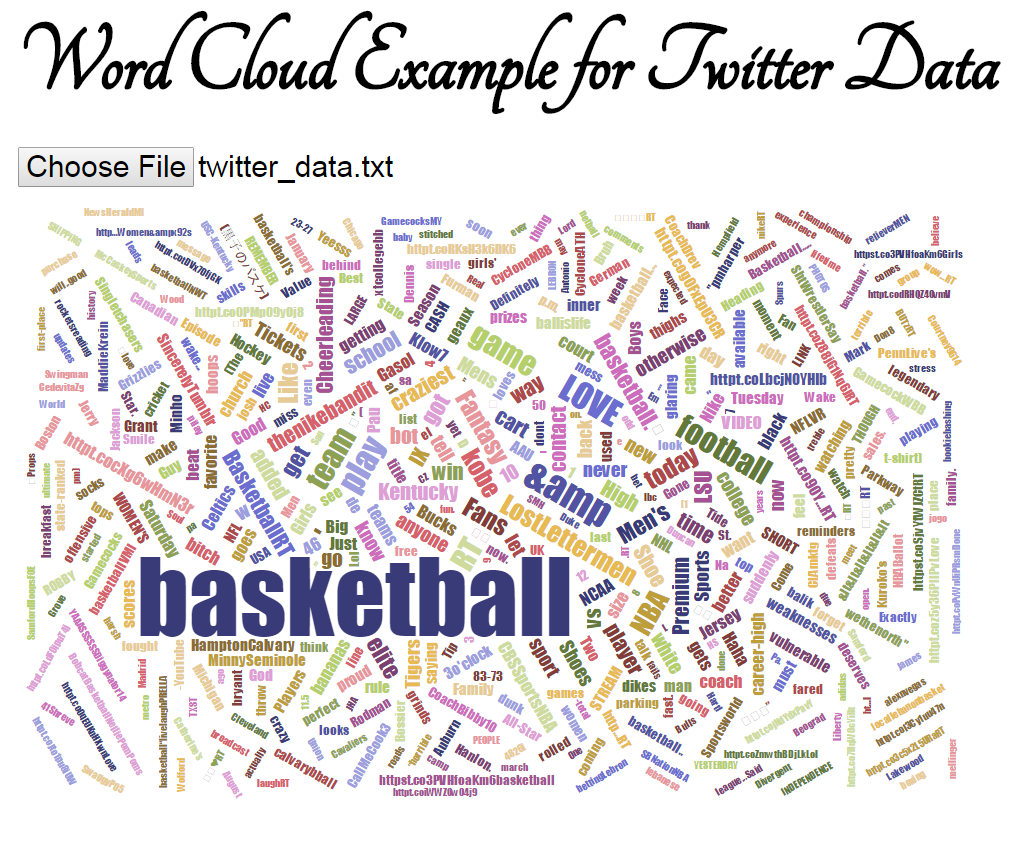
\includegraphics[width=0.8\textwidth]{word_cloud.png}
  \caption{Word cloud for \href{http://nymph332088.github.io/CIS4340/labassignments/Lab2/twitter_data.txt}{tweets data}}
  \label{fig:wordcloud}
\end{figure}

\end{document}